\documentclass[tikz,border=5pt]{standalone}

\usepackage{comment}

\usepackage{graphicx}
\usepackage{tikz}
\usetikzlibrary{positioning,fit}

\usepackage[scaled]{helvet}
\renewcommand{\familydefault}{\sfdefault}


\begin{document}
\begin{tikzpicture}[
  font=\sffamily,
  node distance=1.2cm and 2cm,
  every node/.style={inner sep=0,outer sep=0}
]

%--- Top box: prior+resources plot + "Ground truth (L2 loss)" label
\node (topPlot) {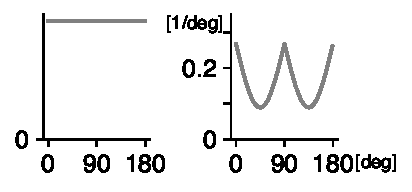
\includegraphics[width=0.55\textwidth]{figures/CounterfactualModel_VIZ_Components_Fig2.py_5_UNIFORM_STEEPPERIODIC_2_0_10.0_180.pdf}};
\node[above=0.05cm of topPlot, anchor=center] (temp0) {};
\node[left=1.7cm of temp0, anchor=center] (prior-gt) {\large prior};
\node[left=1.2cm of prior-gt, anchor=center, yshift=0.7cm](label-a){\Large a};
\node[right=2.8cm of prior-gt, anchor=center] (resources-gt) {\large resources};
\node[right=0cm of topPlot.north, anchor=south,  yshift=0.5cm, align=center] (gtlabel) {\large Ground truth (L$_2$ loss)};
\node[rotate=90, below=-0.8cm of topPlot.west,  xshift=-0.4cm](prob-label){probability};

%% Draw a dotted rectangle around both the plot and the label
%\node[draw, dotted, thick, rounded corners, inner sep=0.3cm,
%      fit=(topPlot)(gtlabel)] (topBox) {};

\node[right=8.5cm of label-a, anchor=center](label-b){\Large b};
\node[right=10cm of label-a, anchor=center, align=left, yshift=-0.2cm](model-likelihood){\large model\\ \large likelihood};
\node[below=0.3cm of model-likelihood, anchor=north,xshift=-0.4cm,yshift=0.2cm] (nllPlot)
  {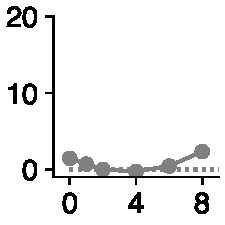
\includegraphics[width=0.25\textwidth]{figures/evaluateCrossValidationResults_Synthetic_Gardelle_NonF_Figure3.py_SimulateSynthetic_Parameterized_OtherNoiseLevels_Grid_VarySize.py_180_2_5_N10000_UNIFORM_STEEPPERIODIC.txt_RelativeLF.pdf}};
\node[below=0.01cm of nllPlot, anchor=north, xshift=0.3cm] (exponent-label)
  {exponent};

%--- Second row: L0 loss (left), L2 loss (right)
\node[below=0.8cm of topPlot.south, anchor=north, xshift=-0.5cm] (l0Label) {\large L$_0$ loss};
\node[left=2cm of l0Label, anchor=east, yshift=-0.2cm](label-c){\Large c};
\node[below=0.3cm of l0Label, anchor=north] (l0Plot)
  {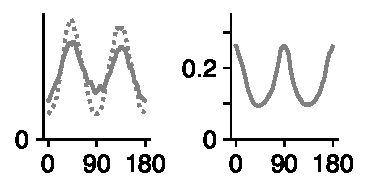
\includegraphics[width=0.42\textwidth]{figures/RunSynthetic_FreePrior_ZeroTrig_OnSim_VIZ_OnlyModel_OtherNoiseLevels_Figure3.py_SimulateSynthetic_Parameterized_OtherNoiseLevels_Grid_VarySize.py_180_2_5_N10000_UNIFORM_STEEPPERIODIC.txt_0_0_10.0_180.pdf}};


\node[right=6cm of l0Label, anchor=center] (l2Label) {\large L$_2$ loss};
\node[left=2cm of l2Label, anchor=east, yshift=-0.2cm](label-d){\Large d};
\node[below=0.3cm of l2Label, anchor=north] (l2Plot)
  {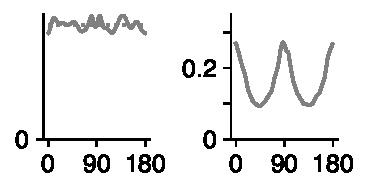
\includegraphics[width=0.42\textwidth]{figures/RunSynthetic_FreePrior_CosineLoss_OnSim_VIZ_OnlyModel_OtherNoiseLevels_Figure3.py_SimulateSynthetic_Parameterized_OtherNoiseLevels_Grid_VarySize.py_180_2_5_N10000_UNIFORM_STEEPPERIODIC.txt_2_0_10.0_180.pdf}};


%--- Third row: L4 loss (left), L8 loss (right)
\node[below=0.9cm of l0Plot.south, anchor=north] (l4Label) {\large L$_4$ loss};
\node[left=2cm of l4Label, anchor=east, yshift=-0.2cm](label-e){\Large e};
\node[below=0.3cm of l4Label, anchor=north] (l4Plot)
  {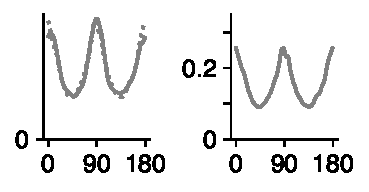
\includegraphics[width=0.42\textwidth]{figures/RunSynthetic_FreePrior_CosineLoss_OnSim_VIZ_OnlyModel_OtherNoiseLevels_Figure3.py_SimulateSynthetic_Parameterized_OtherNoiseLevels_Grid_VarySize.py_180_2_5_N10000_UNIFORM_STEEPPERIODIC.txt_4_0_10.0_180.pdf}};

\node[right=6cm of l4Label.east, anchor=center] (l8Label) {\large L$_8$ loss};
\node[left=2cm of l8Label, anchor=east, yshift=-0.2cm](label-f){\Large f};
\node[below=0.3cm of l8Label, anchor=north] (l8Plot)
  {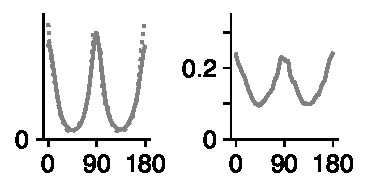
\includegraphics[width=0.42\textwidth]{figures/RunSynthetic_FreePrior_CosineLoss_OnSim_VIZ_OnlyModel_OtherNoiseLevels_Figure3.py_SimulateSynthetic_Parameterized_OtherNoiseLevels_Grid_VarySize.py_180_2_5_N10000_UNIFORM_STEEPPERIODIC.txt_8_0_10.0_180.pdf}};


\end{tikzpicture}

\begin{comment}
python3 evaluateCrossValidationResults_Synthetic_Gardelle_NonF_Figure3.py SimulateSynthetic_Parameterized_OtherNoiseLevels_Grid_VarySize.py_180_2_5_N10000_UNIFORM_STEEPPERIODIC.txt

python3 CounterfactualModel_VIZ_Components_Fig2.py 2 0 10.0 180 1000 UNIFORM STEEPPERIODIC 5

python3 RunSynthetic_FreePrior_CosineLoss_OnSim_VIZ_OnlyModel_OtherNoiseLevels_Figure3.py 8 0 10.0 180 SimulateSynthetic_Parameterized_OtherNoiseLevels_Grid_VarySize.py_180_2_5_N10000_UNIFORM_STEEPPERIODIC.txt
#python3 RunSynthetic_FreePrior_CosineLoss_OnSim_VIZ_OnlyModel_OtherNoiseLevels_Figure3.py 6 0 10.0 180 SimulateSynthetic_Parameterized_OtherNoiseLevels_Grid_VarySize.py_180_2_5_N10000_UNIFORM_STEEPPERIODIC.txt
python3 RunSynthetic_FreePrior_CosineLoss_OnSim_VIZ_OnlyModel_OtherNoiseLevels_Figure3.py 4 0 10.0 180 SimulateSynthetic_Parameterized_OtherNoiseLevels_Grid_VarySize.py_180_2_5_N10000_UNIFORM_STEEPPERIODIC.txt
python3 RunSynthetic_FreePrior_CosineLoss_OnSim_VIZ_OnlyModel_OtherNoiseLevels_Figure3.py 2 0 10.0 180 SimulateSynthetic_Parameterized_OtherNoiseLevels_Grid_VarySize.py_180_2_5_N10000_UNIFORM_STEEPPERIODIC.txt
python3 RunSynthetic_FreePrior_ZeroTrig_OnSim_VIZ_OnlyModel_OtherNoiseLevels_Figure3.py 0 0 10.0 180 SimulateSynthetic_Parameterized_OtherNoiseLevels_Grid_VarySize.py_180_2_5_N10000_UNIFORM_STEEPPERIODIC.txt
#python3 RunSynthetic_FreePrior_L1Loss_OnSim_VIZ_OnlyModel_OtherNoiseLevels.py 1 0 10.0 180 SimulateSynthetic_Parameterized_OtherNoiseLevels_Grid_VarySize.py_180_2_5_N10000_UNIFORM_STEEPPERIODIC.txt

\end{comment}

\end{document}

